\documentclass{MYZJUMCM}
\usepackage{fontspec}
\setControlNumber{8889888}
\setContestType{MCM}

\setProblemLetter{B}

%字体
\setmainfont{Times New Roman}
\setBibFilename{McmTexExample}
\setPaperTitle{My Title}
\setSummary{This paper showes the usage of latex class HZNUMCM and gives most used examples for mathematical typeset. This paper can also be used as a handbook for typing latex. We give the pdf file and the source code file.

This HZNUMCM class file comes from  easymcm, a latex .sty package and a simple MCM Contest Report Template for basic users from oringinal template by latexstudio, <latexstudio@hotmail.com> improved by youjiarui189 (xjtu-blacksmith), <yjr134@163.com>.

This document also pick many pages from the not so not introduction to Latex \cite{tobias}, so that one can search quickly. 
}

\begin{document}
\showSummarySheet
\showContents
\section{Basic usage of the HZNUMCM class}
\subsection{Basic document structure for using HZNUMCM class}

The basic .tex file structure is as the following and comment for each corespending line is listed.
\begin{lstlisting}[style=latexstyle]
	\documentclass{HZNUMCM}.    % class choose
	\setControlNumber{8889888}  % set Control Number
	\setContestType{MCM}        % contest type, only MCM or ICM allowed
	\setProblemLetter{B}        % choose problem A,B,C,D,E or F
	\setBibFilename{McmTexExample} % set bib file, without dot and suffix
	\setPaperTitle{My Title}    % set your title
	\setSummary{summary}        % define summary
	\begin{document}
		\showSummarySheet       % show summary, the first page.
		\showContents           % show contents
		\section{aaaa}
			...
		\section{bbbb}
			...
			...
		\showReferences         % show references
	\end{document}
\end{lstlisting}
\subsection{Process from source files to target .pdf} 
Usually, the process can be executed as following:
\begin{itemize}
\item Type what you think in the .tex file, following the Latex syntax. 
\item xelatex several times, biblatex one time and then xelatex several times again.
\end{itemize}


% subsection subsection_name (end)
\section{Introduction to mathematical typeseting within Latex}

We choose mathematical typeseting from \cite{tobias}.



\section{Some complements}
We put the source code of the HZNUMCM latex class file and this file on the gitHub \url{https://github.com/hznu-maguochun/HZNUMCM}, so that one use it can understand it. Any one, who want to use or improve it, is welcome. This class file also gives an idea about how to make a formatted file.
\showReferences

 


%\includepdf[pages=57-86,offset=0cm 0.5cm]{lshort.pdf}
\end{document}
